In this chapter, we describe the approach which we have adopted to create the dynamic benchmark of executable python software. The overall workflow of the approach is shown in the Figure \ref{fig:overall_approach}.
With the provided approach, our benchmark aims to achieve the properties as listed below.
\begin{itemize}
    \item \textbf{Large-scale} The benchmark should comprise tens of real-world open-source projects, allowing users to evaluate their analyses on a wide range of code.
    \item \textbf{Diverse} The benchmark should contain projects from a diverse range of application domains that reflect the state of today's Python ecosystem.
    \item \textbf{Ready-to-run} There should be a single interface to run each project in the benchmark, making it easy for users to set up and execute the entire benchmark.
    \item \textbf{Ready-to-analyze} To enable dynamic analyses, the executions of all projects in the benchmark should be set up to be analyzed.
    \item \textbf{Compositional} To help users understand the behavior of specific projects or even individual test cases, it should be easy to run subsets of full benchmark.
    \item \textbf{Long-term} The benchmark should be built using commonly used tools and formats, e.g., pip and Docker, to ensure its longevity.
    \item \textbf{Extensibility} The benchmark should be easily extensible, allowing users to add, remove or update the tools, frameworks and projects.  
\end{itemize}

We start with a large corpus of open source python projects listed in the awesome-python project (Section \ref{approach:corpus of python projects}). The projects are selected from this large corpus based on the selection criteria as described in Section \ref{approach:selection criteria}. This selection gives us a collection of python projects in the form of GitHub URLs and certain flags in a text file (Section \ref{approach:list of projects}). The collection of projects in the text file and bash scripts are used for automated installation of projects and their dependencies (Section \ref{approach:bash scripts}) providing us with a set of installed python projects and an environment which is ready to be used by developers and researchers as described in Section \ref{approach:collection of projects}. Orchestration (Section \ref{approach:python script}), with the help of python scripts provide a single command line interface access to the benchmark.  This access interface (Section \ref{approach:access interface}) incorporates  analysis frameworks like LExecutor, DynaPyt and PyCG into the benchmark for execution of various tasks such as dynamic analysis, trace file generation, and static call graph generation respectively (Section \ref{approach:analysis framework}). The benchmark containing the installed projects along with its access interface is packaged and exported as a docker container for use by researchers and developers (Section \ref{approach:packing and exporting}).

\begin{figure}[ht]
\centering
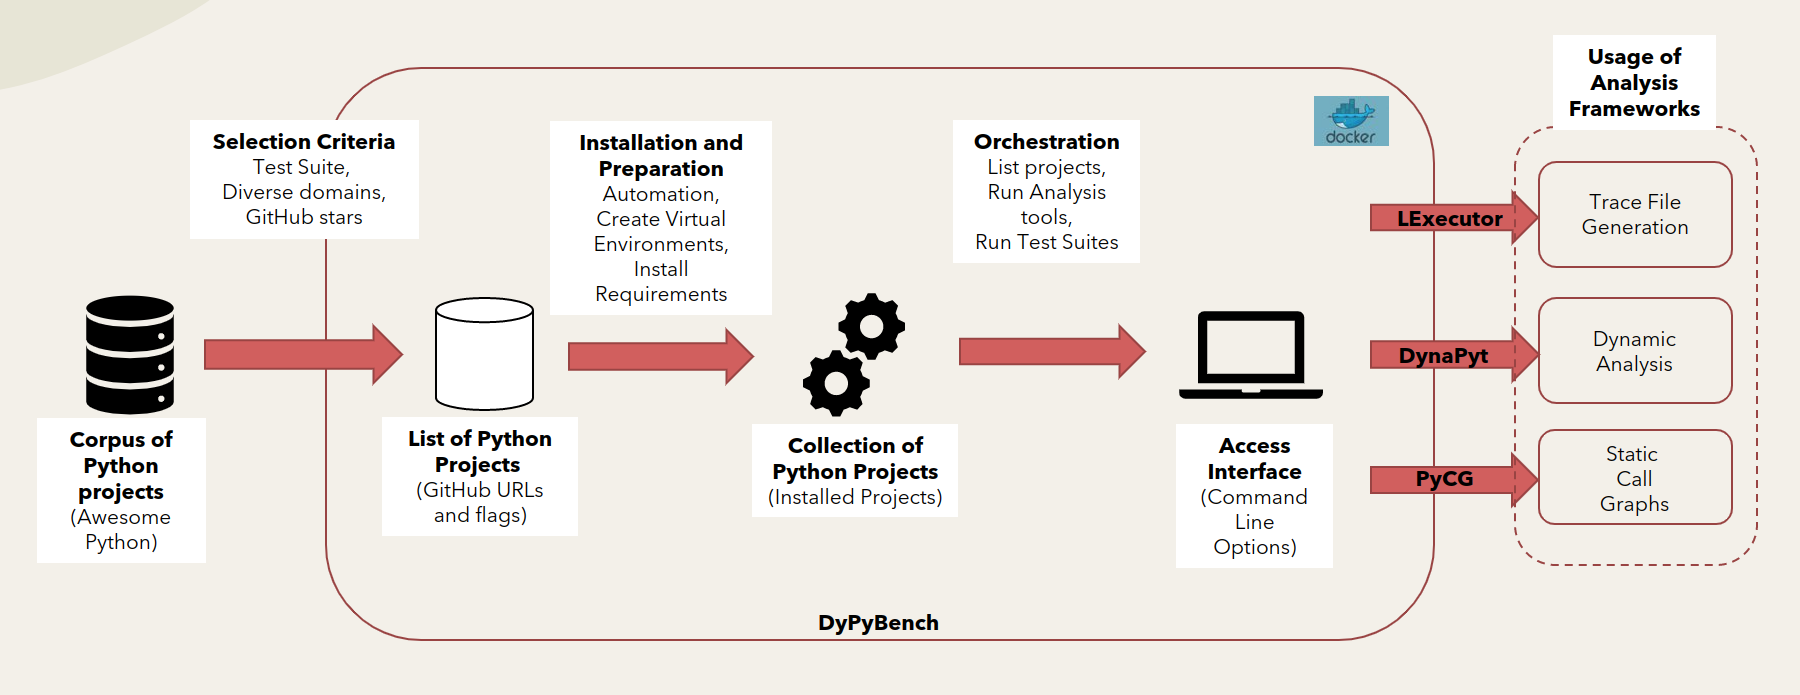
\includegraphics[width=1\linewidth]{figures/approach/DyPyBench2.png}
\caption[Approach]{\label{fig:overall_approach}Overall Approach of DyPyBench}
\end{figure}

\section{Projects Selection}
\label{approach:project selection}

\subsection{Corpus of Python Projects}
\label{approach:corpus of python projects}
Python's ease of use and popularity, as well as the usage in different domains has led to a large number of projects being developed and made available to the community as open source software. GitHub alone contains a lot of public repositories that have python as their primary programming language. It is difficult to classify these projects into their respective domains by looking at each repository. However, there are a few python projects which provide a collection of other python projects such as Awesome Python \cite{awesome_python_github}, Awesome Python Applications \cite{awesome_python_applications_github} and Python Projects \cite{python_projects}. These projects also provide us with a classification for the projects based on the application domains or other criteria. In this work, we use the awesome-python project which contains a list of some of the most useful and interesting open source python projects including libraries, frameworks and software. 
The awesome-python project acts as a corpus for our benchmark as it provides 679 python projects. It further classifies these projects into 92 main categories, out of which some of the categories can be further divided into sub-categories. Some of the categories and the number of projects in those are listed in table \ref{table:awesome-python}. 
Appendix \ref{appendix:awesome python projects} provides more details on the various categories and number of projects in each category provided by awesome-python project.

\begin{table}[ht]
    \centering
    \begin{tabular}{lc}
    \hline
    \textbf{Category} & \textbf{Number of Projects}\\
    \hline
    Admin Panels    & 9\\
    Code analysis   & 18\\
    Computer vision & 7\\
    Deep Learning   & 7\\
    Documentation   & 3\\
    Files   & 7\\
    GUI development & 16\\
    Robotics    & 2\\
    Task Queues & 5\\
    Web Frameworks  & 5\\
    \hline
    \end{tabular}
    \caption{Project Categories (Awesome Python)}
    \label{table:awesome-python}
\end{table}

\subsection{Selection Criteria}
\label{approach:selection criteria}
The corpus of python projects provides us with a large number of projects to choose from the diverse application domains.
However, since a benchmark cannot contain too many projects due to space and other constraints, we need to restrict the projects which will make the benchmark helpful for its intended purpose.   
The selection criteria does exactly this for our benchmark, i.e., it makes the benchmark large scale and diverse by selecting 50 python projects from the available corpus.
For the selection process of our benchmark, there are three main criterion namely diverse domain, test suite execution with pytest and GitHub stars.
The criteria of diverse domain ensures that we select the projects which belong to different categories as described in the section \ref{approach:corpus of python projects}.
Since, in this work we are creating a dynamic benchmark we focus on the projects for which we can perform execution. Test suites provide us with files that can easily execute the code using testing libraries such as pytest, unittest, flake8, etc. As a result we include the criterion of the presence of test suites. However, we limit the execution of tests via pytest as it is a popular testing library and is also used by the DynaPyt framework for analysis.
The number of stars a project has on GitHub is an indication of how popular and well-regarded it is in the community. More stars generally mean more people have found the project useful and interesting, and it has a larger user base and community of contributors. Since a benchmark must contain useful and meaningful projects, we include the criterion of a minimum 500 GitHub stars for the project selection. This is also a common practice among benchmarks in other languages such as Java Microbenchmark Harness (JMH) and Google Benchmark. 

\subsection{List of Python Projects}
\label{approach:list of projects}
Applying the selection criteria as described in section \ref{approach:selection criteria}, we gather 50 open-source python projects from diverse application domains. Each project has its own set of dependencies and source code structure.
Since, our goal is to install and setup these projects for use in our benchmark we need some generic way of handling these differences of setup, installation and execution of projects. 
In this work, we handle the differences with the help of a text file that contains the GitHub URL, flag and test details for each of the 50 projects. This file can be referred to as the collection text file and each line in this file contains the details of one project in the benchmark. Furthermore, we can easily add, modify, delete more projects to and from this file which makes the benchmark extensible for projects.
The GitHub URL helps us in obtaining the source code of the project needed by the analysis tools and frameworks. 
The flag indicates the presence or absence of requirements file in order to install dependencies for the project. If this flag indicates the presence of the requirement file then the collection text file also contains the path of the requirements file. The need for the path arises due the different structure of source code for individual projects.
 The collection text file also specifies the path of the test directory or the test file to be run using the pytest library.
 Table \ref{table:list of projects} shows the structure of the collection text file containing the list of 50 python projects in the benchmark.
 The first row indicates the entry with the presence of requirements file, while the second row indicates the entry without the requirements file.

\begin{table}[ht]
    \centering
    \begin{tabular}{llll}
    % \hline
    % \textbf{GitHub URL} & \textbf{Flag} & \textbf{Requirement File} & \textbf{Test Path}\\
    \hline
    https://github.com/test/test-project.git    & rt    & src/requirement.txt   & src/tests\\
    https://github.com/test/test-project.git    & t    & src/tests\\
    \hline
    \end{tabular}
    \caption{List of Projects (Collection Text File Structure)}
    \label{table:list of projects}
\end{table}

\section{Benchmark Preparation}
\label{approach:benchmark preparation}

\subsection{Installation and Preparation of Projects}
\label{approach:bash scripts}
With the collections text file as described in section \ref{approach:list of projects}, the 50 chosen python projects are ready to be installed and setup in the benchmark. Since, we have the GitHub URL and requirement file flag available via the collections text file, a number of steps are performed for each project to install the project with its dependencies. These steps are listed below:
\begin{itemize}
    \item \textbf{Get the source code :} The list contains open source projects having their source code on GitHub which is cloned to a specific folder in the benchmark. 
    \item \textbf{Create virtual environment :} The virtualenv \cite{virtualenv} package creates a virtual environment which avoid dependency conflicts and system pollution, dodge installation lockups and minimize reproducibility issues \cite{Why_Virtual_Env}.
    \item \textbf{Install project and its dependencies :} The pip package manager \cite{pip_package_manager} installs the project and its module dependencies from the requirements.txt file or the setup.py file.
\end{itemize}
Manually performing these steps for each of the 50 projects is a mundane and repetitive task and may result in frustrating errors.
Such tasks can be automated with the help of bash scripts which can run specific commands on the command line in a sequential order.
Since the above mentioned steps need to be executed in a sequential fashion for each project we need to use loops in the bash script to handle repetition.
The differences in the installation steps such as additional dependencies and installation with setup.py or source code can be handled with conditionals.

\subsection{Collection of Python Projects}
\label{approach:collection of projects}
By following the steps outline in section \ref{approach:bash scripts}, we have a group of 50 projects that are installed and ready to be used in the benchmark.
This collection of projects forms the pool of projects which can be analyzed using the frameworks such as DynaPyt, LExecutor, and PyCG.
The collection is stored in a folder with numbered sub-folders for each project, which makes it easy to use.
Each project has its dependencies installed within its own python virtual environment, which also includes pytest and any other necessary dependencies to run the project's test suite.
To ensure the long-term use of the benchmark, a duplicate of the specific project from the collection is created whenever the analysis needs to be performed. 
This ensures that the projects retain their source code and dependencies in the original folder, which may change due to the nature of the python and open-source ecosystems.
The collection also ensures that the projects are always available for use and do not require re-installation each time they are needed.   

\subsection{Integrated Analysis Frameworks}
\label{approach:analysis framework}
With the collection of projects as described in section \ref{approach:collection of projects}, our benchmark aims to be ready-to-analyze these projects.
In order to achieve this, three analysis frameworks are integrated in our benchmark namely, DynaPyt, LExecutor and PyCG. However, other analysis frameworks and tools can be easily added to the benchmark.
Each of the three frameworks provided in this work helps with a different usage scenario.
\subsubsection{DynaPyt}
DynaPyt is a dynamic analysis framework that provides hooks for a variety of runtime events in multiple layers of abstraction.
Users can create arbitrary dynamic analysis by implementing relevant hooks \cite{DynaPyt2022}. Some of the builtin dynamic analysis include SimpleTaintAnalysis, TraceAll and MLMemoryAnalysis.
In this work, we use DynaPyt for generating run-time call graphs.
\subsubsection{LExecutor}
LExecutor is a learning-guided approach for executing arbitrary code snippets in an under-constrained way.
The key idea is to let a neural model predict missing values that otherwise would cause the program to get stuck, and to inject these values into the execution.
For example, LExecutor injects likely values for otherwise undefined variables and likely return values of calls to otherwise missing functions \cite{LExecutor_2023}. 
In this work, we use LEexecutor to generate trace files to prepare a data-set to train and validate neural model of LExecutor.
\subsubsection{PyCG}
PyCG is a practical Python call graph generator that generates call graphs for Python code using static analysis.
It efficiently supports higher-order functions, twisted class inheritance schemes, automatic discovery of imported modules for further analysis, and nested definitions \cite{PyCG_2021}.
In this work, we use PyCG to generate static call graphs for the collection of projects.

\section{Artifact Packing and Interface}
\label{approach:artifact packaging and interface}

\subsection{Orchestration}
\label{approach:python script}
The collection of projects and the analysis frameworks as described in section \ref{approach:collection of projects} and section \ref{approach:analysis framework} provides us with the dynamic benchmark. 
However, we need a way to make this benchmark easily accessible for the users.
Orchestration of the projects and the analysis frameworks with the help of python script creates this easy access to the benchmark.
Python scripts are user-friendly and offer extensive support for both standard and third-party libraries that can be utilized for automating tasks, data processing, and analysis.
They are also easily extensible, allowing for the addition of new features without interfering with previous functionality.
These scripts can be triggered from the CLI and can accept command line options.
In this work, the python script acts as the primary entry point and triggers the execution of other scripts via the subprocess module \cite{python_subprocess}.
This script offers functionalities such as listing the projects in the benchmark, running test suites and executing the analysis frameworks on the collection of projects.  
The script accepts a variable number of arguments, which makes the benchmark compositional i.e., the script can perform the operation on all the projects or a subset of projects in the benchmark. 

\subsection{Access Interface}
\label{approach:access interface}
Orchestration on the collection of projects as described in section \ref{approach:python script} provides us with a single command line access interface to the operations of the benchmark.
In this work, the single command line interface access makes the benchmark ready-to-run and ready-to-analyze via this interface.
The access interface provides various alternatives to the end user specified by the command line options.
The available options to this interface are provided in the table \ref{table:access interface options}, where the first column specifies the option and the second column provides description of its usage.
Some of these options such as dynapyt\_instrument, dynapyt\_run, lex\_instrument, lex\_test and pycg allow to specify a variable number of projects which makes the benchmark highly versatile.

\begin{table}[ht]
    \centering
    \begin{tabular}{ll}
    \hline
    \textbf{Option} & \textbf{Description}\\
    \hline
    list    & List the project number, name and GitHub URL\\
    test    & Run test suite of specified projects\\
    save    & Save standard output and error to file specified\\
    timeout & Timeout in seconds for commands\\
    update\_dynapyt\_source   & Clone or update source code of DynaPyt\\
    update\_lex\_source   & Clone or update source code of LExecutor\\
    dynapyt\_instrument  & Instrument files for DynaPyt\\
    dynapyt\_file    & Specify file to use for instrumentation of DynaPyt\\
    dynapyt\_analysis    & Specify the analysis to perform for DynaPyt\\
    dynapyt\_run & Execute DynaPyt analysis for specified projects\\
    lex\_instrument  & Instrument files for LExecutor\\
    lex\_file    & Specify file to use for instrumentation of LExecutor\\
    lex\_test    & Execute LExecutor for specified projects\\
    pycg    & Execute PyCG for specified projects\\
    \hline
    \end{tabular}
    \caption{Access Interface (Command Line Options)}
    \label{table:access interface options}
\end{table}

\subsection{Packing and Export}
\label{approach:packing and exporting}
The collection of projects, analysis frameworks and the access interface as described in sections \ref{approach:list of projects} through \ref{approach:access interface} together constitute the benchmark in this work.
In order to make the benchmark easy to access and setup, it is packaged and exported along with all its components, such as python scripts, bash scripts, analysis frameworks and collection of projects inside a docker container.
Docker is a platform that allows applications to be wrapped and executed within a container, which provides a loosely isolated environment that eliminates the need to rely on the host's existing software.
This container is then exported as an image on the dockerhub \cite{docker_hub} repository, which can be easily imported and run as a container by users on any major operating system. 
By sharing the docker image, everyone can access the same container that works in the same way \cite{Docker_2022}.
This approach of using docker provides the users with a complete and easily analyzable benchmark, and also ensures the longevity as the image is available ling after the project's release.
Additionally, this approach allows for easy extensibility of the benchmark, as users can take it as a base image and make changes according to their needs, such as adding more analysis tools or modifying the collection of projects.
